
\chapter{Data-Centric Language Constructs}

Super-languages must provide mechanisms that allow new language constructs
to be defined for representing data. The new constructs must make
it easy to represent the required data structures. This chapter shows
how new language constructs can be defined for records and trees.


\section{Simple Records\label{sub:Simple-Records}}

This section provides an introduction to the definition of a new language
construct. All aspects of a new construct are covered, but the construct
is rather simple since it supports data records consisting of fields
with names and values. The record construct is an example of an integrated
language construct since the field values can be any language construct
supported by XOCL. Since XOCL is itself open-ended, this allows record
field values to be expressed as any language construct including records
and those constructs we have not even thought of yet!

Our requirement is for a database containing records. Each record
has a collection of fields with a name and a value. A database may
be filtered by supplying it with a predicate that expects a record.
The result is a new database containing all those fields that satisfied
the predicate.

\begin{figure}
\begin{center}

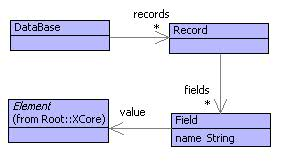
\includegraphics[width=12cm]{LanguageEngineering/DataModelling/Images/Records}

\caption{\label{Data Records}A Simple Model Of Data Records}

\end{center}
\end{figure}

It is usual to start off with a data definition for the elements that
are required. Figure \ref{Data Records} shows the contents of a package
called Records. A database consists of a set of records. Each record
is a set of fields. Each field has a value that can be of any data
type (since Element is the super-class of everything).

The next step is to define a concrete syntax for the Record construct
that will synthesize an expresstion whose evaluation produces an instance
of the class Record. The complete grammar for Record is defined below,
followed by a step-by-step description:

\begin{lstlisting}
context Record
  @Grammar extends OCL::OCL.grammar
    Record ::= r = { [| Record() |] } Fields^(r) 'end'.
    Fields(r) ::= r = Field^(r) FieldTail^(r) | { r }.
    Field(r) ::= n = Name '=' e = Exp { 
      [| <r>.addToFields(Field(<n.lift()>,<e>)) |] 
    }.
    FieldTail(r) ::= ',' Fields^(r) | { r }.
  end
\end{lstlisting}When a syntax construct starts with the token @Record, XMF looks for
a grammar associated with the class Record. If it finds one then the
grammar should have a rule with the name Record; this rule is the
starting point for the parse.

The rule named Record defined above, creates an expression named r
that will create a new record when evaluated. The expression r is
passed as an argument to the rule named Fields. Once fields has completed
its parse, the keyword 'end' is expected. If successful, the value
returned by Fields is the result of the parse. So far we have dealt
with the following concrete syntax:

\begin{lstlisting}
@Record
  ???
end
\end{lstlisting}The rule Fields deals with the part labelled ??? above. Fields will
either recognize nothing (an empty record) or will recognize a sequence
of fields separated by commas. If there are fields, the rule uses
Field followed by FieldTail, otherwise the rule returns the supplied
expression r. Note the repeated use of the variable r in the rule
Fields. It is used as a formal argument, a modified variable, an actual
argument and in the body of an action.

A field is defined by the rule Field, it is a name n, followed by
= followed by an expression e. If successful, it synthesizes an expression
that adds a field to the supplied record r. So far, the following
can be recognized:

\begin{lstlisting}
@Record
  name = "Fred"
end
\end{lstlisting}FieldTail is used to allow more than one field to be recognized. A
FieldTail is either a comma followed by some fields (notice how the
record expression is threaded through so that it is continually built
up), or is nothing. 

The grammar is complete and the following records can be recognized
and the appropriate expressions synthesized:

\begin{lstlisting}
@Record
  name = "Fred",
  age = 35
end
\end{lstlisting}which synthesizes the following expression:

\begin{lstlisting}
Record()
  .addToFields(Field("name","Fred"))
  .addToFields(Field("age",35))
\end{lstlisting}
\section{Trees}

Information often naturally forms a tree structure where each component
of information is related to several children. Think of company structures:
responsibilities from CEO downwards or groupings from the board down.
Trees are often used to model physical entities such as cars where
a car consists of a body, an engine, electrical system, interior etc.
and where a body consists of doors, a windscreen etc.

Trees are useful when we want to organise a model in terms of parent-child
relationships which may be physical containment or may be logical
groupings (think of nested sets). This section gives an example of
a language for expressing trees for classification.

Consider a collection of bank records that are to be classified with
respect to awarding a loan. The first step to awarding the loan is
to determine an income threshold. If the applicant does not have an
annual salary of four times the loan amount then the loan is denied.

The next step is to consider the current debt position of the applicant.
If the applicant has debts of more than �10K then the loan is denied.
If they have debts of �5 - �10K then the loan application is referred
otherwise the application might be awarded.

Finally, if the applicant has an account with the bank, then the loan
is awarded otherwise it is referred.

%
\begin{figure}
\begin{center}

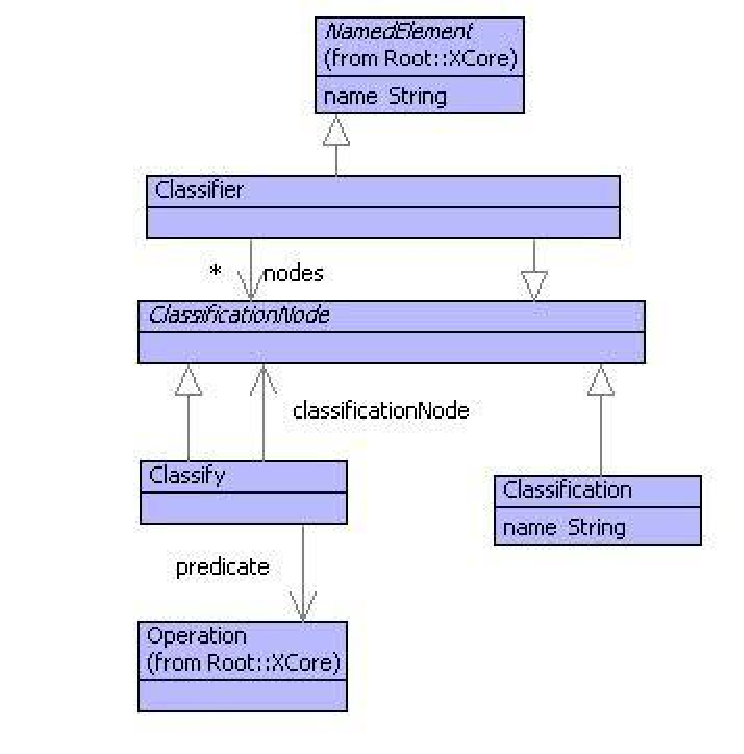
\includegraphics[width=12cm]{LanguageEngineering/DataModelling/Images/Classifications}

\caption{\label{Classification-Tree-Model}Classification Trees}

\end{center}
\end{figure}


Figure \ref{Classification-Tree-Model} shows a simple model of a
classification tree. A classifier is a named element (so that it can
be put in name spaces and then referred to from elsewhere). A classification
is a property of some data (for example Award the loan, Deny the loan
or Refer the loan). Finally, a classify, is something that applies
a predicate to some data to determine whether the classification given
by the classificationNode applies.

To construct a classification tree, proceed as follows. Start with
a classifier node. Its child nodes, will be classify nodes with disjoint
predicates. The child node of a classifier node will be either a classification
or another classifier. Proceed with the tree until all categories
are classified.

The following example shows a classifier for a loan:

\begin{lstlisting}
@Operation loan(bank,amount)
  @Classifier Loan
    @Classify(applicant)
      applicant.lookup("salary") * 4 > amount
      @Classifier
        @Classify(applicant)
          applicant.lookup("debt") >= 10000
          @Classification Deny end
        end
        @Classify(applicant)
          applicant.lookup("debt") < 10000 and
          applicant.lookup("debt") >= 5000
          @Classification Refer end
        end
        @Classify(applicant)
          applicant.lookup("debt") < 5000
          @Classifier
            @Classify(applicant)
              applicant.lookup("bank") = bank
              @Classification Award end
            end 
            @Classify(applicant)
              applicant.lookup("bank") <> bank
              @Classification Refer end
            end
          end
        end
      end
    end
    @Classify(applicant)
      applicant.lookup("salary") * 4 <= amount 
      @Classification Deny end
    end
  end
end
\end{lstlisting}The operation loan accepts a bank and a loan amount. It returns a
classifier for the amount. The classifier first checks that the applicant
has an adequate annual salary for the required loan. If this condition
is not met then the application is denied. Otherwise, the amount of
debt is analysed. There are three outcomes: the first denies the application;
the second refers the application and the third analyses the bank
of the applicant. If the bank of the applicant is the same as that
receiving the application then the load is awarded otherwise the application
is referred.

The operation loan may be applied to any number of banks and loan
amounts. In each case it returns a different classifier.

The classification language is defined by adding a grammar to each
of the appropriate classes in the classification model. Each class
gets its own grammar so that the classification language is not fixed.
The classification language is integrated into XOCL and the components
of the language are extensible (new types of classifier node can be
defined later and they can be integrated with no changes to the existing
components).

Classification is the simplest grammar:

\begin{lstlisting}
@Grammar
  Classification ::= n = Name 'end' { 
    [| Classification(<n.lift()>) |] 
  }. 
end

\end{lstlisting}since it recognizes a name and synthesizes an instance of the appropriate
class. Classify, involves capturing XOCL expressions and is defined
as follows:

\begin{lstlisting}
@Grammar extends OCL::OCL.grammar
  Classify ::= '(' n = Name ')' e = Exp c = Exp 'end' { 
    [| Classify(@Operation(<n>) <e> end,<c>) |] 
  }.
end
\end{lstlisting}Notice that Classify synthesizes an operation definition whose argument
name is supplied in tthe classify definition. This is a standard way
of capturing executable code (in this case e) within synthesized elements.
The body of the operation, e, may refer to any variables that are
in scope. The argument n is deliberately placed in scope and allows
the body to refer to data that will be supplied by the instance of
Classify.

Classification involves sequences of XOCL expressions (an arbitrary
number of child classification nodes); it is defined as follows:

\begin{lstlisting}
@Grammar extends OCL::OCL.grammar
  Classifier ::= n = OptName c = Classifications 'end' {
    [| Classifier(<n.lift()>,<c>) |] 
  }.
  Classifications ::= e = Exp cs = Classifications { 
    [| <cs> ->including(<e>) |] 
  } | { [| Set{} |] }.
  OptName ::= Name | { "anon" }.
end
\end{lstlisting}The key aspect of the definition above is how the set of child classification
nodes is constructed using the Classifications rule. This recognizes
nothing, in which case it synthsizes an expression that creates the
empty set; or, it recognizes an expression e (a child node definition)
followed by more classifications cs and then synthesizes an expression
that adds e to cs. This is an example of a recursive rule%
\footnote{The rule is right recursive because the recursive use of Classifications
occurs after some input must be consumed. XMF does not support left
recursion where Classifications could occur on the left since this
would lead to Classifications calling itself without consuming any
input.%
}

with a base case that creates an empty set.

\begin{itemize}
\item Types and simple type checking (Dynamic - type check the classifiers.
vs Static)
\item Rendering configuration data.
\end{itemize}

